\subsection{QuizziPedia::Back-End::App::Models}
\subsubsection{Informazioni generali}
\label{QuizziPedia::Back-End::App::Models}
\begin{figure}
	\centering
	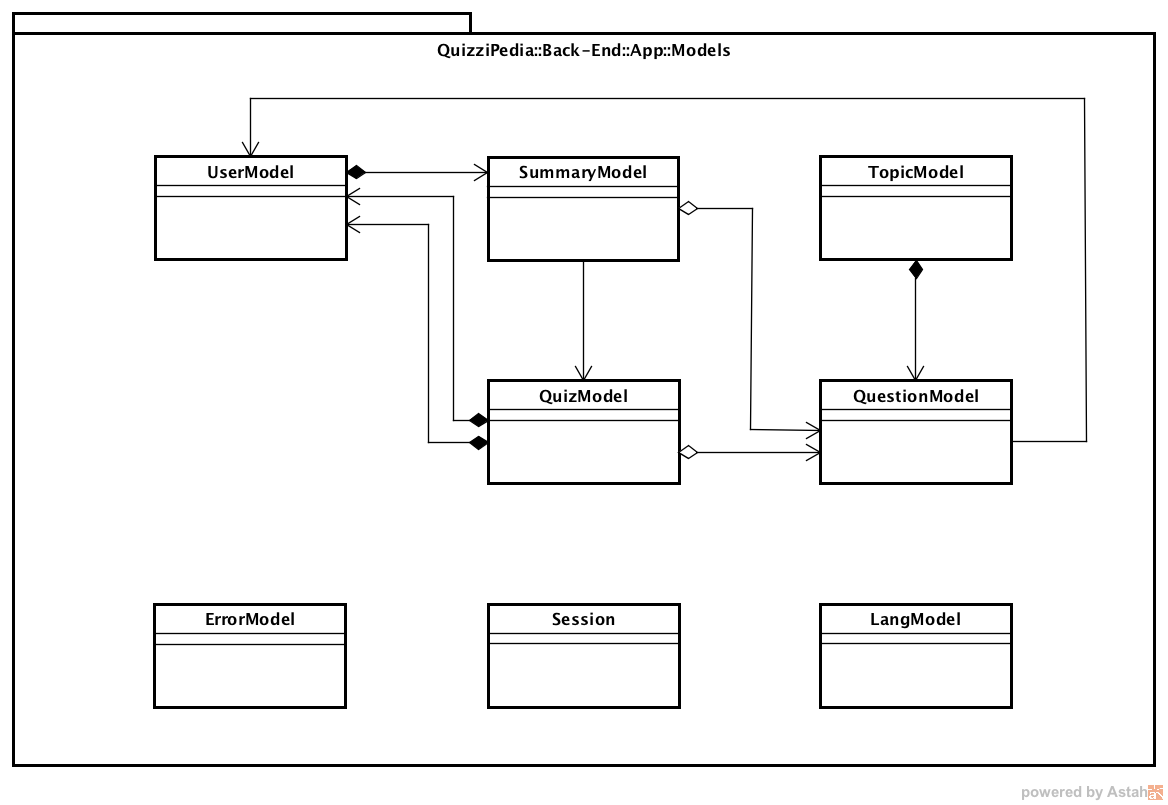
\includegraphics[scale=0.45]{UML/Package/QuizziPedia_Back-End_App_Models.png}
	\caption{QuizziPedia::Back-End::App::Models}
\end{figure}

\subsubsection{Classi}

\paragraph{QuizziPedia::Back-End::App::Models::UserModel}
\begin{itemize}
	\item \textbf{Descrizione} \\
	Classe che modella la creazione e la gestione dei dati utente
	\item \textbf{Utilizzo} \\
	Viene utilizzata per rappresentare i dati degli account dei vari utenti dell’applicazione. Si interfaccia alla libreria Mongoose per la creazione dello schema e dei relativi metodi statici o di istanza.
	\item \textbf{Relazioni con altre classi} \\
		\begin{itemize}
			\item \textbf{IN QuestionModel} \\
			Questa classe rappresenta i dati delle domande create dai vari utenti.
			\item \textbf{IN QuizModel} \\
			Questa classe rappresenta i dati dei questionari creati dai vari utenti.
			\item \textbf{IN QuizSummaryModel} \\
			Questa classe rappresenta i dati dei questionari creati dai vari utenti.
		\end{itemize}
	\item \textbf{Attributi} \\
		\begin{itemize}
			\item \textbf{- userSchema: Schema} \\
			Questo campo dati rappresenta lo schema Mongoose dell'utente QuizziPedia. Lo schema prevede i seguenti attributi:
			\begin{itemize}
				\item 
					name di tipo String, rappresenta il nome  dell'utente registrato;
				\item 
					surname di tipo String, rappresenta il cognome  dell'utente registrato;
				\item 
					email di tipo String, rappresenta l'email  dell'utente registrato;
				\item 
					userImg di tipo String, rappresenta il path della foto profilo dell'utente registrato;
				\item 
					userType di tipo String, rappresenta la tipologia dell'utente registrato;
				\item 
					username di tipo String, rappresenta l'username con cui viene identificato l'utente all'interno dell'applicazione;		
				\item
					password di tipo String, rappresenta la password associata all'utente,    appositamente codificata mediante l'algoritmo bcrypt;  		
				\item
					statistics di tipo Array Mixed, contenente i seguenti attributi:
				\begin{itemize}
					\item
						topic di tipo String, identifica la statistica derivante dalle esercitazioni effettuate dall'utente in un determinato argomento; 
					\item
						 topicLevel di tipo Number, identifica il livello di preparazione dell'utente in un determinato argomento;
					\item
						correctAnswers di tipo Number, identifica il numero di risposte corrette date dall'utente riguardanti domande di un determinato argomento; 
					\item						
						 totalAnswers di tipo Number	, identifica il numero di risposte totali date dall'utente riguardanti domande di un determinato argomento.		
				\end{itemize}		
				\item 
					levelUsers di tipo Number, identifica il livello dell'utente;				
				
				\item
					quizSummaries di tipo Array, contiene oggetti di tipo ObjectId, che rappresentano i riferimenti agli identificativi nel database dei questionari svolti dall'utente;		
			\end{itemize}	
		\end{itemize}	
	\item \textbf{Metodi} \\
		\begin{itemize}
		\item
		- generateHash(password: String): String
		Effettua l'hashing della stringa password se non è già stata criptata tramite campo salt per evitare attacchi di tipo rainbow. \\
		\textbf{Parametri} \\
			\begin{itemize}
			\item
				 password: String
				Rappresenta la password dell'utente.
			\end{itemize}
		\item
		- validPassword(password: String): String 
		Effettua la validità della password inserita comparandola con la password criptata.	\\
		\textbf{Parametri} \\
			\begin{itemize}
			\item
				 password: String
				Rappresenta la password dell'utente.
			\end{itemize}
		\end{itemize}	
\end{itemize}